\documentclass[pdftex]{article}
\usepackage[T1]{fontenc}
\usepackage[utf8]{inputenc}
\usepackage{graphicx}
\usepackage{caption}
\usepackage{titling}

\setlength{\droptitle}{-15em}
\title{PHYS 721 Homework 4}
\author{Nick Tyler}
\date{}


\begin{document}
\maketitle
\begin{enumerate}
	\item Three Breit-Wigner curves for the decay $\phi \rightarrow K^{+} K^{- }$ are plotted on the same graph. 
		The first, in green, is the relatavistic Breit-wigner. The second, in red, is the Non-Relatavistic
		Breit-Wigner curve.  These curves look almost identical which implies that the decay products, 
		in this case $K^{+}$ and $K^{-}$, leave with very little energy. The third curve, in blue,
		shows the decay with an energy dependent width.  This line is pushed to the right because at
		low energy the width is close to the nominal width while at higher energy, and larger $\beta$,
		the width increases.\\
		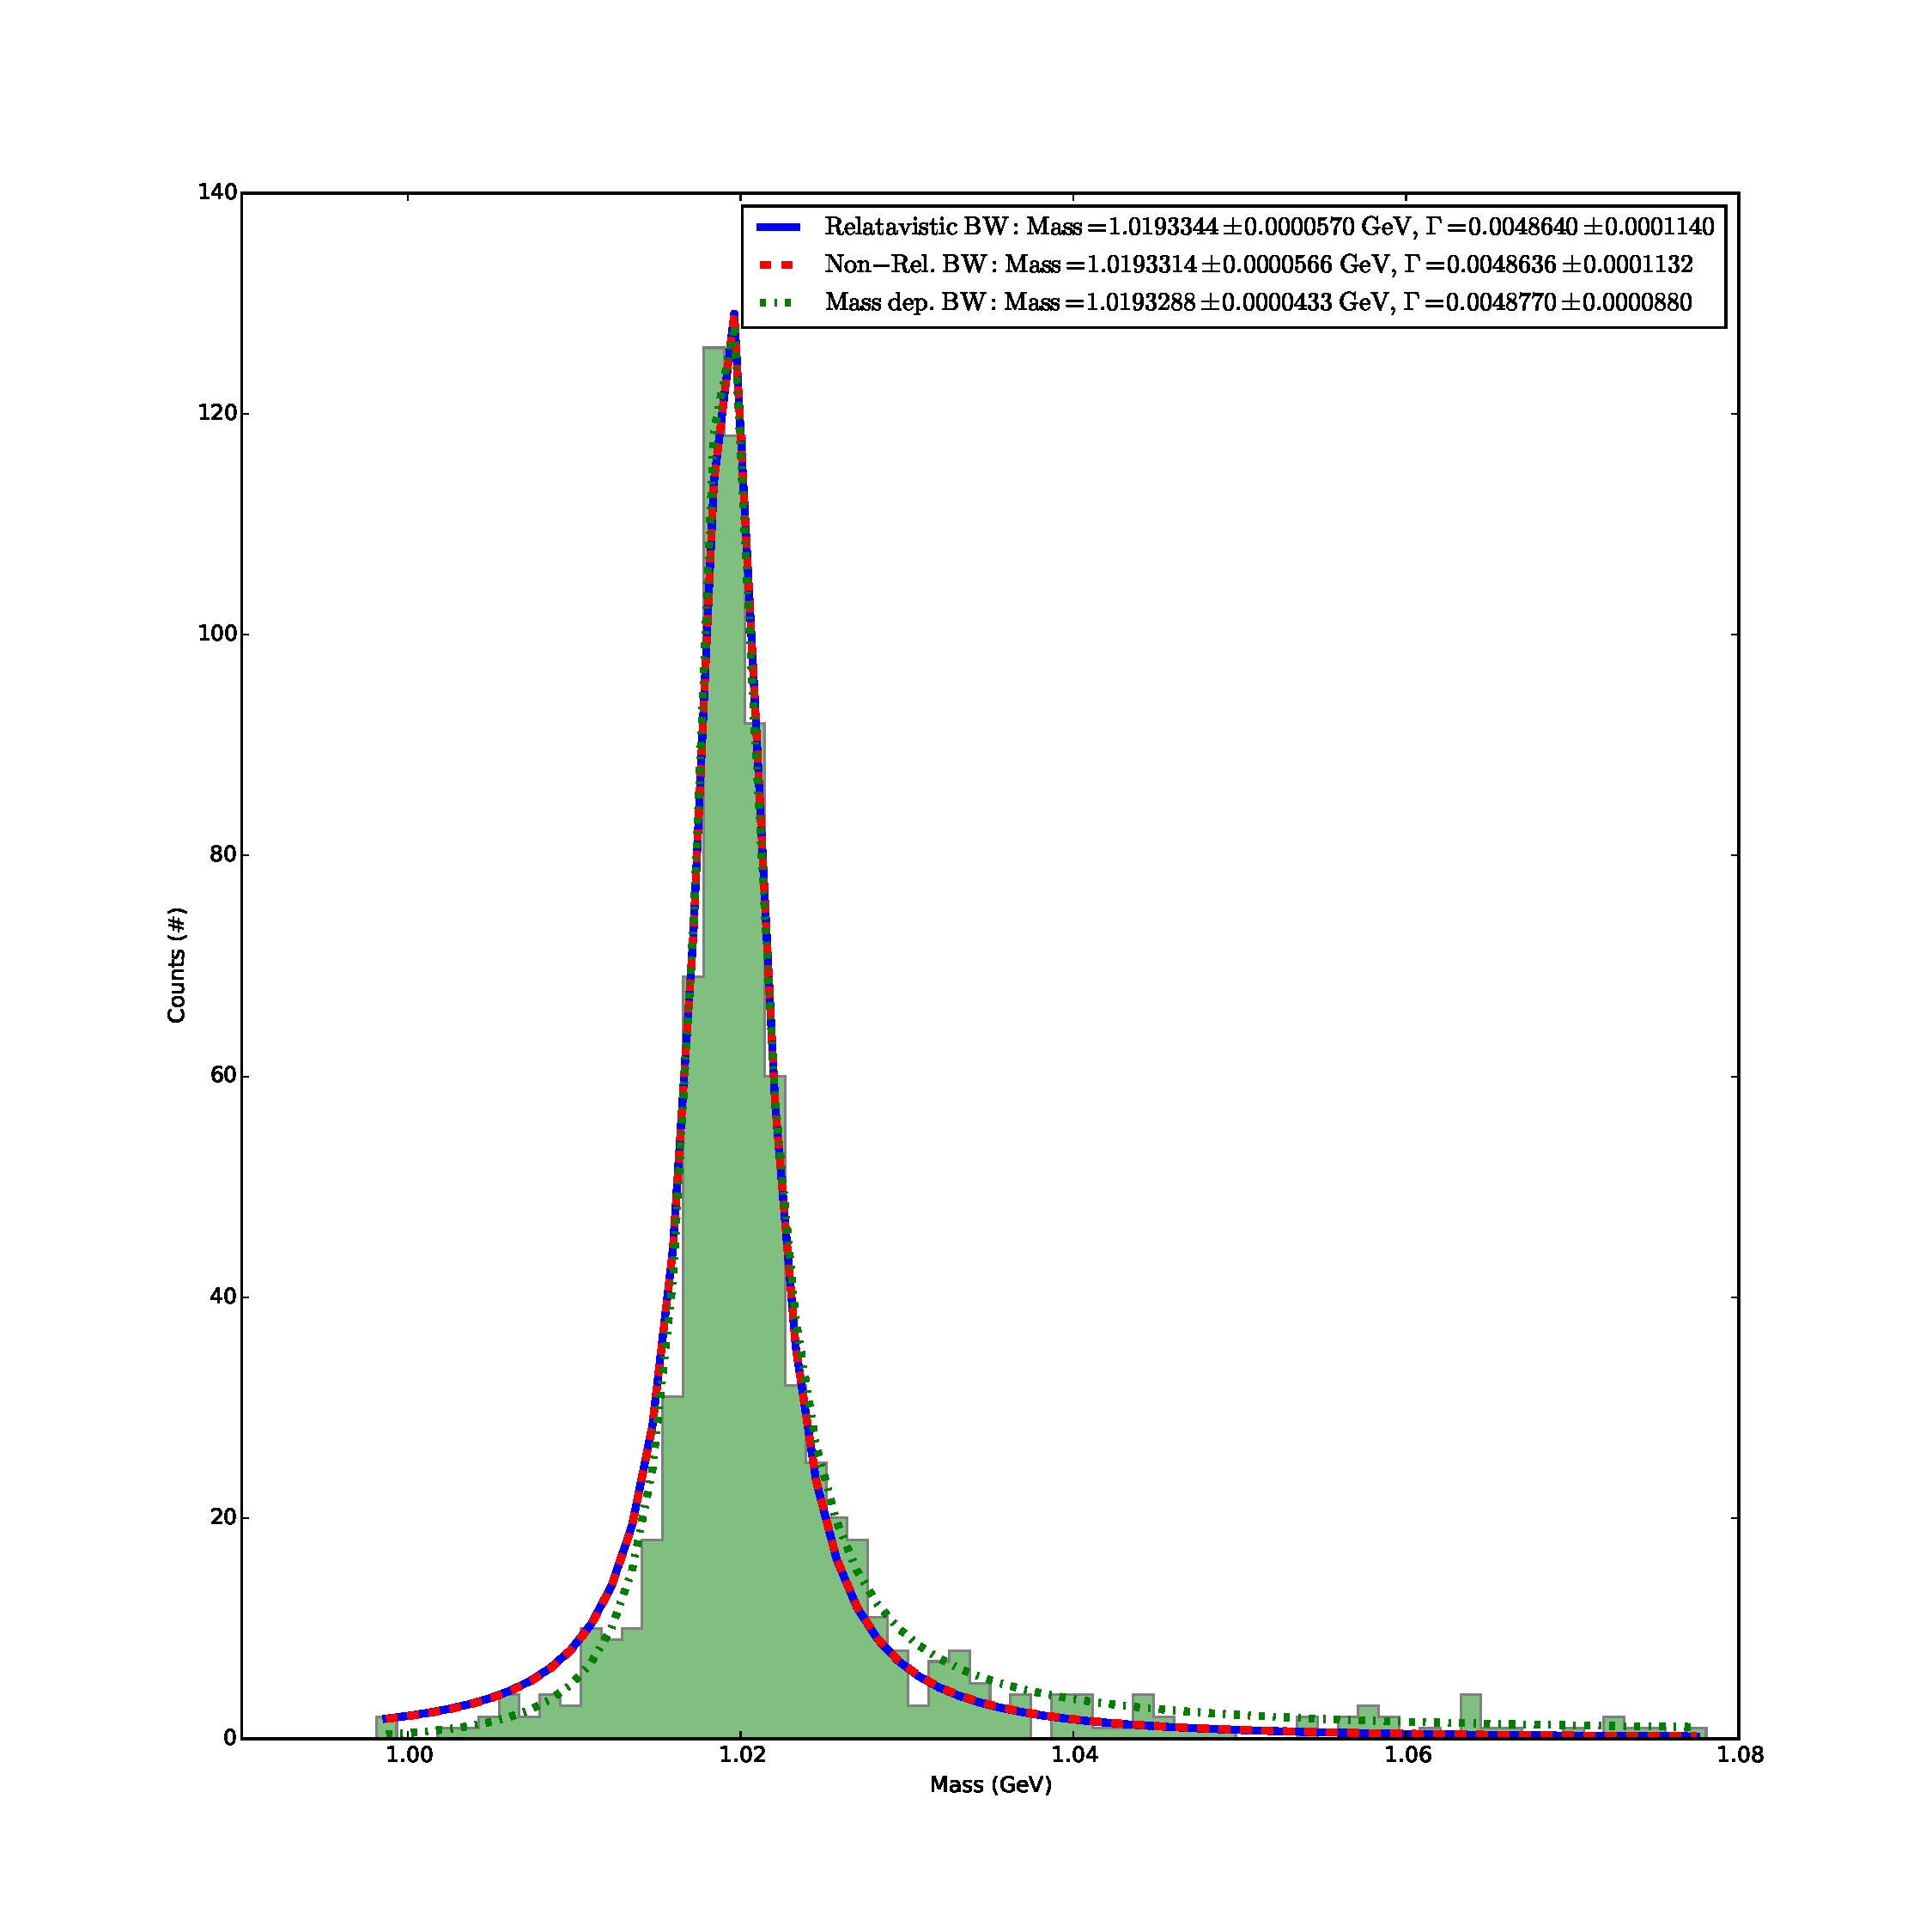
\includegraphics[scale=0.35]{Problem_1.pdf}\\
		\captionof{figure}{Three Breit-Wigner curves for, $\phi \rightarrow K^{+} K^{- }$}

\end{enumerate}

\end{document}
